\chapter{Background}
\label{ch:back}
In this chapter we present the background details required for our heap intensive data dependence analysis.
\section{Programming Model}
Each and every node of a heap recursive data structure can be 
accessed by access path, which is defined as pointer variable or variable 
followed by link fields, similar to languages like Fortran 90, C. As an example, 
a node \emph{N} can be accessed by either pointer variable \emph{ptr} or pointer variable  
followed by link fields like \emph{ptr}\rtarrow{$f_1$}\rtarrow{$f_2\cdots{f_k}$}, 
where $f_1$, $f_2$, $\cdots$, $f_k$ are pointer fields of heap structure. All statements 
in the program are pre-processed to provide normalized binary access paths, 
defined as pointer variable followed by single pointer field reference like 
\emph{ptr\rtarrow{f}}. The model of the programming language to be analysed 
closely resembles the model of imperative language like C. We are interested in 
analysing only heap related statements. Here we enumerate with details the basic statements 
operating on heap. Note that,  
arithmetic operations of pointers, as in C, are not allowed.
\begin{itemize}
\item Heap allocating statements :

\begin{itemize}
\item {\tt p = malloc()} : A new heap object is allocated, which is pointed to by pointer \ttf{p}. 
Hence, this statement is called as memory allocation statement. 
\end{itemize}

\item Pointers assigning statements :

\begin{itemize}
\item {\tt p = q} : Pointer {\tt p} points to the same heap location as pointed 
to by {\tt q}. It inherits all the relations and properties of {\tt q}. Hence 
this statement results in {\tt p} and {\tt q} to be alias.
\item {\tt p = q$\rightarrow$f} : This statement makes pointer {\tt p} to access 
the heap object which is accessible by pointer {\tt q} through the pointer field 
{\tt f}. This type of statement is mainly used to traverse the links of recursive 
dynamic data structure. 
\item {\tt p = NULL} : This statement assigns pointer variable \ttf{p} to null, such that \ttf{p} 
does not point to any heap location. 
\end{itemize}

\item Link defining/ structure updating statements :

\begin{itemize}
\item {\tt p$\rightarrow$f = NULL} : This statement breaks the link \ttf{f} emanating from the heap node pointed 
to by pointer variable \ttf{p}. After the execution of the statement \ttf{p} can not reach any other heap node 
through link field \ttf{f}.
\item {\tt p$\rightarrow$f = q} : This statement first breaks the link \ttf{f} of the heap node 
pointed to by \ttf{p} and then resets \ttf{f} such that \ttf{p} through link field \ttf{f} 
access the same heap node pointed to be pointer variable \ttf{q}. 
\end{itemize}

\item Heap reading/ writing statements : 

\begin{itemize}
\item {\tt $\cdots$ = p$\rightarrow$data} : Data field of the heap node pointed to 
by pointer variable \ttf{p} is accessed. Hence this statement is used to read the 
data value of heap node. 
\item {\tt p$\rightarrow$data = $\cdots$} : Data field of heap node, pointed to 
by heap directed pointer variable \ttf{p}, is written by this statement. Hence 
this statement clearly write into heap nodes.
\end{itemize}

\end{itemize}
Our analysis mainly works on those statements which do not update or modify the 
structure of the underlying dynamic data structure. The statements which only traverse the heap structure,   
reading or writing the heap data, are main candidate statements of our dependence analysis. The effects of the statements, which update 
the structure, are captured by shape analysis explained in later section. 
Here we list the statements which 
are handled by our data dependence analysis.
\begin{itemize}
\item {\tt p = q} : aliasing statement.
\item {\tt p = q$\rightarrow$f} : link traversing statement.
\item {\tt $\cdots$ = p$\rightarrow$data} : statement reading heap data.
\item {\tt p$\rightarrow$data = $\cdots$} : statement writing into heap data.
%\item {\tt f($p_1, p_2,\cdots, p_i$)} : 
\end{itemize}
Note that, only single-level of pointer dereferencing is allowed. Other 
than basic heap related statements, heap intensive procedure calls are 
also taken into account. Hence procedure calls, whose parameters point 
to heap nodes,  are also analysed by our analysis.
%%%%%%%%%%%%%%%%%%%%%%%%%%%%%%%%%%%%%%%%%%%%%%%%%%%%%%%%
%%%%%%%%%%%%%%%Dependence Anlaysis%%%%%%%%%%%%%%%%%%%%%%
%%%%%%%%%%%%%%%%%%%%%%%%%%%%%%%%%%%%%%%%%%%%%%%%%%%%%%%%
\section{Dependence Analysis}
Dependence analysis produces the execution order constraints 
between any two statements in a program as described in 
literature~\cite{Muchnick97, Kennedy01Optimizing, Cooper05} etc. 
Two classes of dependences 
are present; (a)Control dependence, where the execution of
a statement depends on the control flow constructs, (b)Data Dependence, 
which arise between two statements \ttf{S} and \ttf{T} if there exists an 
execution path between these two statements and they access or 
modify same data resource. 
%%%%%%%%%%%%%%%%%%%%%%%%%%%%%%%%%%%%%%%%%%%%%%%%%%%%%%%%%%%%%%%%
\subsection{Control Dependence}
Use of control constructs in the program body imposes control dependences.  
Statement \ttf{T} is said to be control dependent on a statement \ttf{S} if 
(a)there exists an execution path from \ttf{S} to \ttf{T} and (b)the execution 
of \ttf{T} depends upon the outcome of statement \ttf{S}. A typical example of such  
dependence is the use of \emph{if-then-else} construct. 
In this case the statements present 
in then or else body can not be executed before the execution of if statement. The 
other examples of such dependence occurs due to control flow construct like 
\emph{while}, \emph{do-while} etc. 
%%%%%%%%%%%%%%%%%%%%%%%%%%%%%%%%%%%%%%%%%%%%%%%%%%%%%%%%%%%%%%%%%%%%%%%
\subsection{Data Dependence}
The other type of dependence is data related dependences~\cite{Maydan91, Lam92, Kennedy01Optimizing}, which can be generally  
classified into following four categories.
\begin{enumerate}
\item Flow (True) Dependence(Read after Write): Statement \ttf{T} is flow dependent on statement 
\ttf{S} if and only if an execution path exists from \ttf{S} to \ttf{T} and 
\ttf{T} reads a data which is already modified by \ttf{S}. 

\item Anti Dependence(Write after Read): Statement \ttf{T} is antidependent on statement 
\ttf{S} if and only if statement \ttf{T} modifies a data which is already read by \ttf{S} and \ttf{S} precedes \ttf{T} in execution. 

\item Output Dependence(Write after Write): Statement \ttf{T} is output dependent on statement 
\ttf{S} if and only if both \ttf{S} and \ttf{T} modify the same data and \ttf{S} precedes \ttf{T} in execution.

\item Input Dependence(Read after Read): A statement \ttf{T} is input dependent on statement 
\ttf{S} if and only if \ttf{S} and \ttf{T} read the same data resource and \ttf{S} precedes \ttf{T} in execution.
\end{enumerate}
Anti and output dependences are false dependence because they can be easily removed by some techniques like variable renaming etc. Input dependence does not impose any dependence as it does not prohibit reordering of instructions. This data dependence 
analysis is extended to tackle dependencies within loops. The next section gives an 
overview of loop dependence analysis. 
%%%%%%%%%%%%%%%%%%%%%%%%%%%%%%%%%%%%%%%%%%%%%%%%%%%%%%
\subsubsection{Loop Dependence}
Loop dependence analysis is a task of determining whether statements present in the 
loop body form dependency within same iteration or across iterations. These
dependences can be categorized into the following classes: 
\begin{enumerate}
\item Loop-carried Dependence : If statement \ttf{S} in one iteration 
depends on statement 
\ttf{T} executed in other iteration. 

\item Loop-independent Dependence : If two statements \ttf{S} and \ttf{T} 
depend on each other in the same iteration of loop. 
\end{enumerate}
Different iterations of loop can be effectively executed in parallel if the 
execution of iterations do not depend on each other, i,e., no loop-carried 
dependence is present. To classify dependence, compiler uses two parameters: 
(a)Distance Vector, which indicates distance between two iterations dependent on each other, (b)Direction vector, indicates the sign of the distance. Based on the direction vector different classes of dependence can be identified. There exist several techniques which are used to tackle loop dependence problem. For 
detect whether a dependence exists, \emph{GCD}, \emph{Lamport}, and 
\emph{Banerjee} tests are most general tests in use. Here we give brief details of \emph{GCD} and \emph{Lamport} tests. 
%
\subsubsection*{GCD Test}
A simple and sufficient test for the absence of loop carried 
dependences is the GCD test~\cite{Kennedy01Optimizing}. 
A loop carried dependency can occur between any two accesses of the same array \ttf{X} 
such as \ttf{X[a*i+b]} and \ttf{X[c*i+d]}, if greatest common divisor of 
\ttf{a} and \ttf{c} divides \ttf{(d-b)}. GCD test has some limitations 
such that it does not consider loop bounds, and does not provide distance and 
direction vectors. Beside these GCD ends up by producing very conservative result as GCD 
of any two integers is often one.
%
\subsubsection*{Lamport Test}
Lamport test~\cite{Lamport1974parallel} is a simple test for index expressions involving a single index variable and 
with a constraint that the coefficients of the index variable must be same. 
In this given scenario, Lamport test can detect both loop-carried and loop-
independent dependencies with both distance and direction vector. Let us consider an example where two accesses of same array such as \ttf{X[a*i + b]} 
and \ttf{X[a*i + c]} form equation 
\[\ttf{a*i_1+b = a*i_2+c \equiv i_2-i_1 = (b-c)/a}\]
If the above equation returns an integer solution then any potential dependence 
is reported. Here dependence distance $\sigma$ is \ttf{(b-c)/a}, if $\sigma$ exists 
between lower and upper bound of the loop. It reports true dependence if $\sigma$>0, anti dependence when $\sigma$<0, and loop-independent dependence if 
$\sigma$=0.

\section{Data Flow Analysis}
Data flow analysis~\cite{Kam76globaldata, Muchnick97, Khedker09} is a technique for gathering particular information at 
each program point of a program. It is inherently flow sensitive, i,e., depends on the order of statements of the program. The flow of analysis mainly fits into one of the following 
three categories: (a)Forward flow analysis, where the flow of analysis 
propagate in the forward direction, and exit or out state of a basic block 
is the function of the entry or in state of it, (b)Backward flow analysis, if the analysis 
move in the backward direction, and the transfer function is applied to the exit 
state yielding the entry state, (c)Bidirectional analysis, if the flow of analysis 
move in both direction. 

Transfer function is mainly the composition of the effects of the statements in the 
basic block. Hence, for each block \ttf{b} transfer function $\ttf{trans_b}$:
\[\ttf{out_b = trans_b(in_b)}\]
%\end{equation}
%\begin{equation}
\[\ttf{in_b = join_{p\in{pred_b}}(out_p)}\]
%\end{equation}
The join operation combines the out or exit states of the predecessors \ttf{p}$\ttf{\in{pred_b}}$ of \ttf{b}, 
returning the entry state of \ttf{b}. 
By solving this set of equations, the entry and/ or exit states are used 
to derive properties at each block boundary. Properties for each statement 
inside a block can also be derived separately by applying proper transfer 
function.

Iterative analysis is one of the most widely used techniques for data flow analysis. 
In case of forward flow analysis, it starts with an approximation of 
the in state for each basic block. The transfer 
function computes the out state for each block from its in state. Again 
the in states are updates by applying the join operations on the out 
states of its predecessors. These steps, excluding initialization, are repeated 
until the the system is stabilized, i,e., reaches fixed-point. The basic 
\emph{round-robin iterative} algorithm for forward flow analysis is given in Figure~\ref{fig:dataIter1}.
%%%%%%%%%%%%%%%%%%%%%%%%%%%%%%%%%%%%%%%%%%%%%%
\begin{figure}
%\hrule
\begin{framed}
{\tt
  \begin{program}{0}
%  \FL fun computeState(In set of stmt:In[Stmt], Statement:Stmt)  \{
  \UNL{0} initialize sets of Entry node
  \UNL{0} \FOR {i $\leftarrow$ 1 to N of basic blocks }
  \UNL{1} initialize the sets of block i
  \UNL{0} change $\leftarrow$ true
  \UNL{0} \WHILE {(change)}
  \UNL{1} change $\leftarrow$ false
  \UNL{1} \FOR {i $\leftarrow$ 1 to N of basic blocks}
  \UNL{2} In[i] = $\bigcup_{j\in{pred[i]}}$(Out[j])
  \UNL{2} Temp = $trans_i$(i)
  \UNL{2} \IF {Out[i] $\neq$ Temp} then 
  \UNL{3} change $\leftarrow$ true
  \UNL{3} Out[i] $\leftarrow$ Temp
  \end{program}
}
\end{framed}
  \caption{Round-robin iterative analysis. \label{fig:dataIter1}}
\end{figure}
%
This classic round-robin iterative algorithm completely sweeps over the graph such that it visits every node in a fixed-order. 
The time bound for this algorithm is high due to the fact that 
the algorithm evaluates some unnecessary computations. 
The \emph{worklist iterative analysis} approach improves on the round-robin iterative algorithm, in 
terms of time, by computing on regions in the graph where information 
is changing. Figure~\ref{fig:dataIter2} outlines the worklist iterative 
algorithm. The algorithm initializes all the nodes accordingly 
and construct an initial worklist. It then continues by removing 
a node from the worklist and updating its data flow information. 
If the value of the node changes, then all the nodes that 
depend on the changed information are added to the worklist. 
These algorithms can also be improved by bit vector technique, 
where data sets are are represented efficiently as \emph{bit vectors}, 
in which bit represents set membership of one particular element.
%%%%%%%%%%%%%%%%%%%%%%%%%%%%%%%%%%%%%%%%%
\begin{figure}
%\hrule
\begin{framed}
{\tt
  \begin{program}{0}
%  \FL fun computeState(In set of stmt:In[Stmt], Statement:Stmt)  \{
  \UNL{0} Worklist $\leftarrow$ $\phi$
  \UNL{0} \FOR {i $\leftarrow$ 1 to N of basic blocks }
  \UNL{1} initialize the sets of block i
  \UNL{1} add i to the Worklist
  \UNL{0} \WHILE {(Worklist $\neq$ $\phi$)}
  \UNL{1} remove a node i from the Worklist 
  \UNL{1} recompute set at node i
  \UNL{1} \IF {new set $\neq$ old set for i then}
  \UNL{2} add each successor of i to Worklist, uniquely
  \end{program}
}
\end{framed}
%\hrule
  \caption{Worklist iterative analysis. \label{fig:dataIter2}}
%\hrule  
\end{figure}
%

\section{Shape analysis}
Shape analysis, as described in literature~\cite{Sagiv99Parametric, Sagiv02parametric, Ghiya96, Sagiv96solvingshape-analysis, Mooly} etc., is used to statically analyse a program to determine various 
informations regarding dynamically allocated recursive 
data structures. It detects various features of the heap structure like interfering and 
sharing of nodes, reachability of heap node, disjointness of structures etc. 
Shape analysis also gives a coarse classification of the shape of underlying recursive heap structure. The shape is classified into one of the 
following three categories: (a)\emph{Tree}, 
in which each node has at most one parent and no two paths can lead to 
same heap node, (b)\emph{DAG}, in which some node has more than one parent 
and two paths can access same node, but it does not contain any cycle, 
(c)\emph{Cycle}, structures having graph theoretic cycle, and a node can be 
potentially accessed by infinite number of paths.
\begin{figure}[htbp]
  \begin{center}
    \scalebox{.85}{\begin{tabular}{@{}c@{} @{}c@{}}
     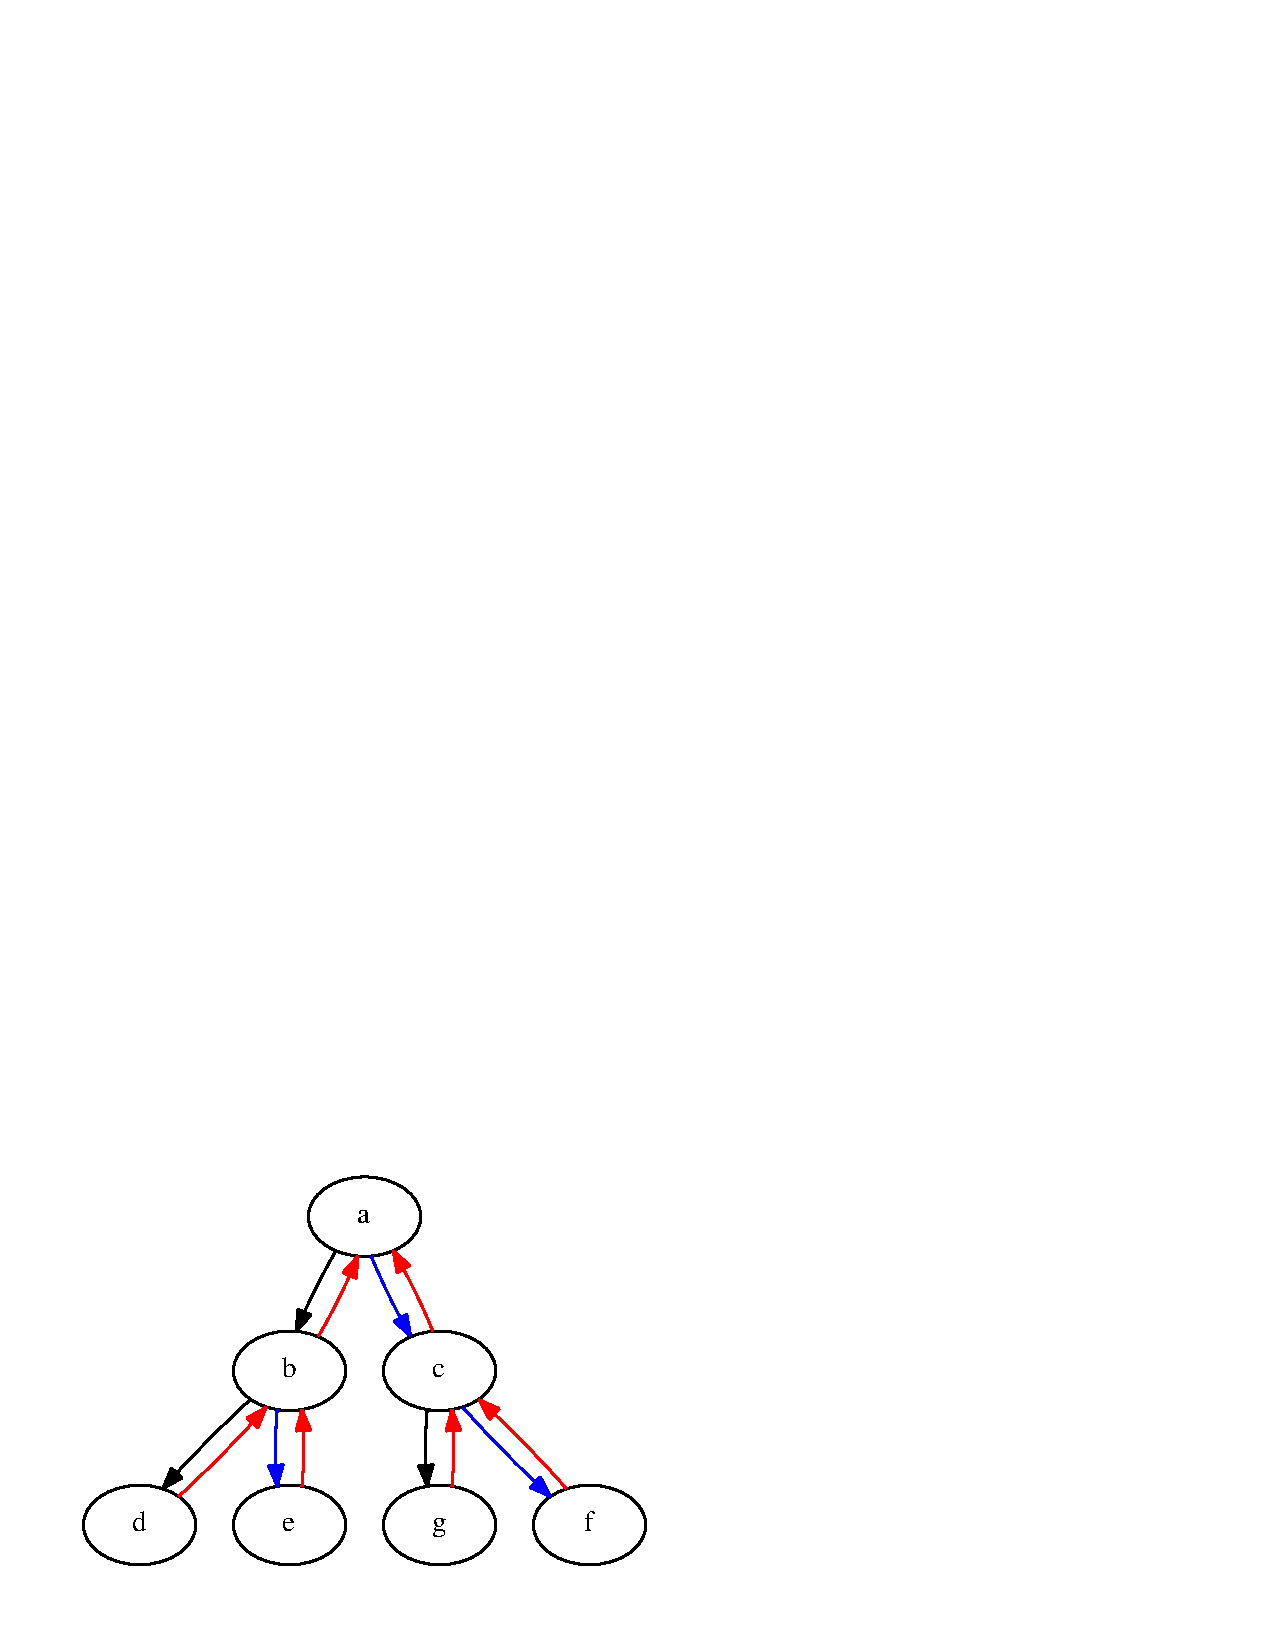
\includegraphics[scale=0.8]{tree} 
     &
      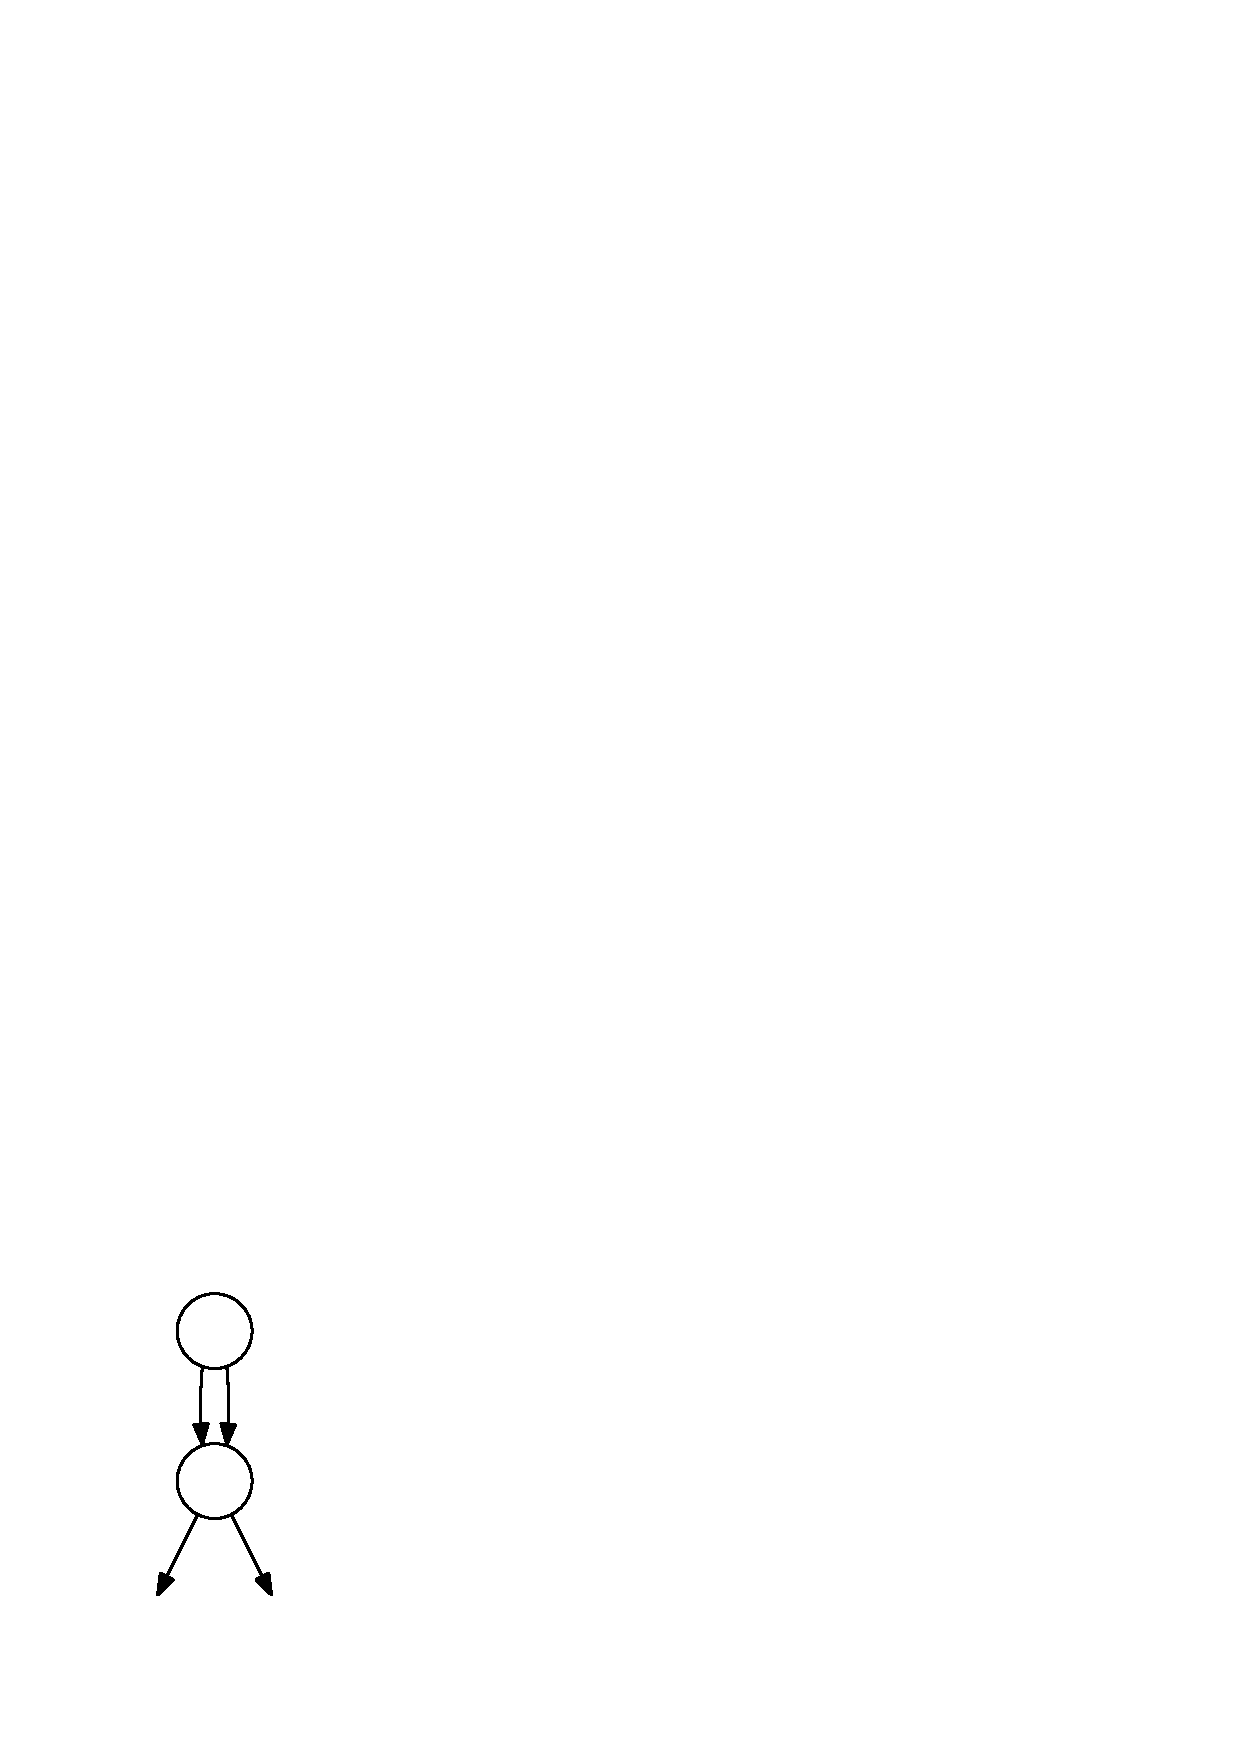
\includegraphics[scale=0.8]{DAG} \\
%      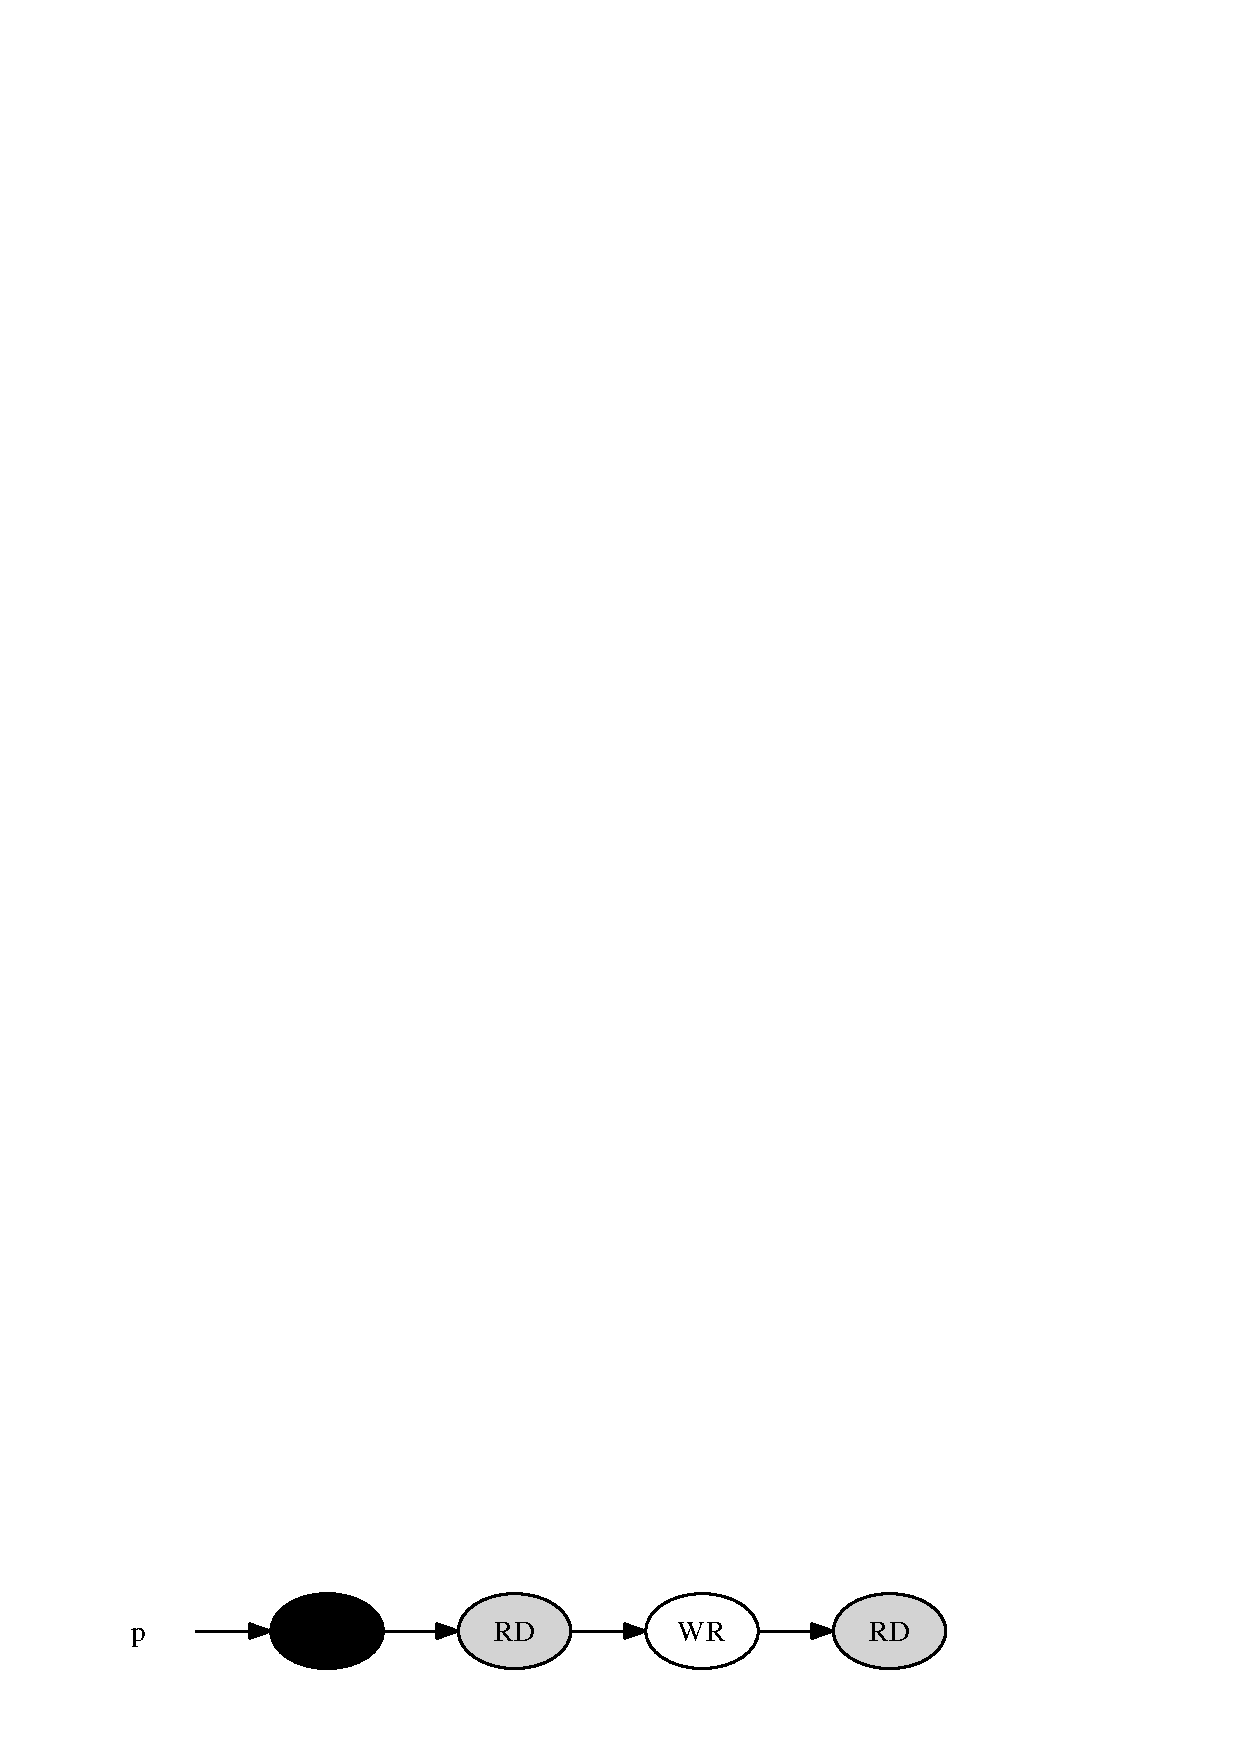
\includegraphics[scale=0.6]{grph_RD_WR} & \\
%    (a) & (b) \\
%   (a) Tree & (b) DAG \\
    \end{tabular}}
  \end{center}
%  \hrule
  \caption{\label{fig:codeStruct} Structure of Tree and DAG}
%\hrule
\end{figure}

The potential for parallelism in programs that use recursive structures arises from the following observation. If the underlying data structure is of type tree, then unrelated sub-trees, $\ttf{T_i}$ and $\ttf{T_j}$, of tree \ttf{T} are guaranteed to share no common storage, hence computation on $\ttf{T_i}$ will not interfere with computation on $\ttf{T_j}$ or any sub-tree of it. For the DAG structure, sub-tree $\ttf{T_i}$ can potentially interfere with sub-tree $\ttf{T_j}$. Hence parallelism can be extracted if and only if it is ensured that the body of code do not access any shared node. Parallelism from cyclic structure can not be easily extracted due to the presence of cyclic nature, hence conservative decision is made. 
%



